%************************************************
\chapter{Konzept}\label{ch:concept}
%************************************************
%
Beim klassischen Client Server Modell muss sich jeder Client Ressourcen über das WAN laden. Abbildung \ref{fig:school} zeigt den typischen Aufbau eines solchen Netzwerks. Sind die geladenen Ressourcen groß kann die WAN Anbindung zu einem Flaschenhals werden. Durch die dadurch resultierenden langen Ladezeiten kann es zu einer starken Einschränkung des Nutzererlebnisses und der Nutzerzufriedenheit kommen.(\emph{\color{red} studie einfügen })

\begin{figure}[!h]
	\centering
	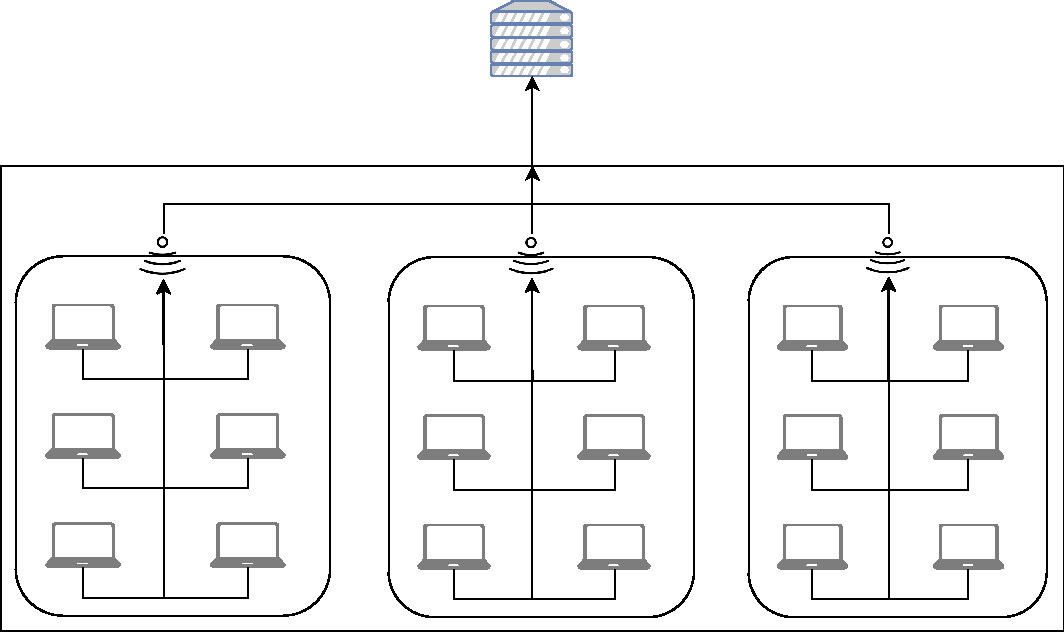
\includegraphics[width=0.8\textwidth]{figures/network_current}
	\caption[A Figure Short-Title]{Netzwerkverkehr in einem herkömmlichen Netzwerk}
	\label{fig:school}
\end{figure}

In den Betrachteten Anwendungsfällen besteht eine hohe zeitlich und inhaltliche Lokalität der Daten. Dies kann genutzt werden um die benötigte Bandbreite zu reduzieren. Dazu soll im Folgenden eine interne Verteilung mittels eines hybriden \pTp Ansatzes untersucht werden. Abbildung \ref{fig:mesh} zeigt exemplarisch den Aufbau eines solchen Netzwerkes. Anstatt das jeder Client sich die Ressource von einem externen Server lädt, lädt nur noch ein Nutzer je Subnetz die Resource über das WAN. Dieser verteilt die Resource dann im internen Netzwerk an andere Clients die diese dann ebenfalls wieder bereitstellen.

Benötigt ein Client eine Resource versucht er zuerst die Resource über sein \pTp Mesh zu laden. Ist dies nicht möglich lädt er sie über einen externen Server. Hat ein Peer eine Resource geladen speichert er sie zwischen und stellt sie für andere Clients bereit.

\begin{figure}[!h]
	\centering
	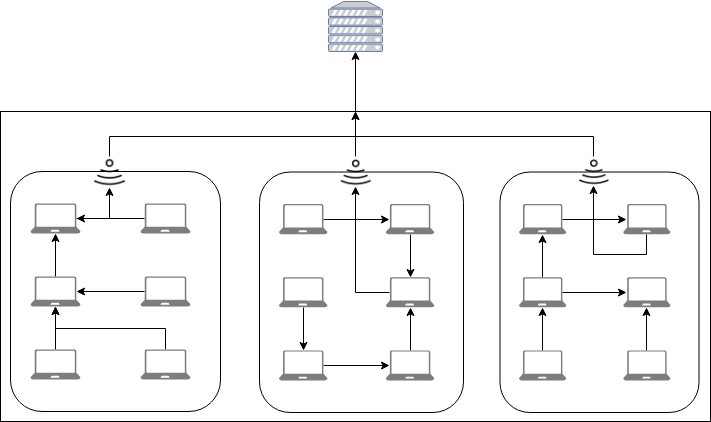
\includegraphics[width=0.8\textwidth]{figures/network_p2p}
	\caption[A Figure Short-Title]{Netzwerkverkehr in einem Peer To Peer CDN}
	\label{fig:mesh}
\end{figure}

Da sowohl im Kontext der Schule als auch bei Unternehmen kein Wissen im Bereich der Computer Administration seitens der Nutzer vorausgesetzt werden kann, wurde ein Ansatz gewählt werden der keine Installation auf Seiten der Nutzer benötigt. Das Nutzererlebnis soll dabei nicht negativ beeinflusst werden. 

% herausstellen das ein plugin entwickelt wird das eingebunden werden kann


% schon geschrieben:
%Genereller Architektur Ansatz
% interne verteilung in subnetzen vs wan verbindung
% Klassische Server architekur mit client und server beschreiben + bild
% p2p mit bild zeigen netzarchitektur
% kommunikation zwischen peer anhand von vereinfachter architektur beschreiben
%	bild peer to peer zwischen browsern ohne service worker
%	peer to peer zwischen browsern
% hybrid p2p CDN ansatz
% keine installation auf clientseite
% domainen wissen soll genutzt werden um clients zu verbinden
% 
%
%
%


%bild schule wie in blockpost?
%
%
%%

% "hybrid p2p cdn"
%konfiguration von subnetzen?

\section{Mesh Zuordnung - Verbinden von Peers}
Im Folgenden werden verschiedene Zuordnungsstragien zur Bildung von Peer Meshes diskutiert. Dazu wird der typische Workload beider Anwendungen analysiert um eine jeweils geeignete Strategie zu wählen. 

\subsection{\schulCloud}
Analyse workload mit grafik

Schulcloud
- Global
einfache umsetzung
Kurs unabhänige assets können geteilt werden
Maximale Mesh größe
Mehrere Meshes nötig
Möglicherweise nicht im Mesh mit relevanten Peers
Maximiert die Anzahl der Peers pro Mesh
Wahrscheinlichkeit für selbes Subnetz eher gering
Funktioniert auch mit wenigen Clients
Ineffektiv wenn viele Clients vorhanden sind

- Schule
Einfache Umsetzung
Funktioniert auch mit wenigen Clients
Relativ hohe trefferrate da schulen selten mehr als 1000 Schüler hat
Max mesh größe um die 256(Chrome)
Relativ wahrscheinlich gleiches Subnetz

- Kurs
Hohe trefferrate
Kleine Meshes
benötigt mehr Clients
Relativ wahrscheinlich gleiches Subnetz --> Daten die das bestätigen

hybride Ansätze:
Zwei priorisierte Meshes Schule und Klasse

Berechnung eines Scores für jeden Peer:
Möglichst viele gemeinsame kurse
Liste von Kursen für jeden Peer
Schnittmenge für jeden peer der online ist bilden
Kardinalität der Menge = Score von Peer
Rechenaufwendig Aber machbar
Beste Trefferrate
Funktioniert wenn wenige und wenn viele Peers anwesend sind

\subsection{Slidesync}
Slidesync ist eine Plattform deren Nutzung stark durch die durchgeführten live Events dominiert wird. Ein Moderator erstellt das Event lädt die notwendigen Assets, z.B. Foliensätze, hoch. Live Events werden für eine bestimmte Zeit festgesetzt und Teilnehmer laden zum start des Events die Seite.\todo{Grafik visits} Ein Großteil des entstandenen Traffics besteht aus HLS Videoseqmenten. Jeder Teilnehmer eines Events benötigt die selben Inhalte.\todo{Grafik traffic} 

Die Peer Meshes in Slidesync werden als voll vermaschte Netzte abgebildet. Da alle Teilnehmer eines Events zu großen Teilen die selben Daten benötigen können sie in dem selben Mesh untergebracht werden. Um zu gewährleisten das sich die Peers im Selben Subnetz befinden teilen sich nur solche ein Peer Mesh die sich in der Selben IP Range befinden. Ein weiterer wichtiger Factor ist der Kommunkationsoverhead der durch das halten von Verbindungen zu vielen Peers entsteht. Deshalb ist es nicht möglich bei größeren Events alle Peers im selben Peer Mesh unter zu bringen. Deshalb werden Sub Meshes gebildet in denen sich eine maximale Anzahl an Peers befinden können. 

Abbildung \ref{fig:mesh-slidesync} zeigt eine beispielhafte Aufteilung von Peer Meshes für ein Event. Für Netzwerk A und B werden jeweils zwei Meshes erzeugt und nur solche Clients werden miteinander verbunden die sich auch im Selben Subnetz befinden. Jedes Netzwerk wird wiederum in zwei Sub-Meshes unterteilt.

\begin{figure}[!h]
	\centering
	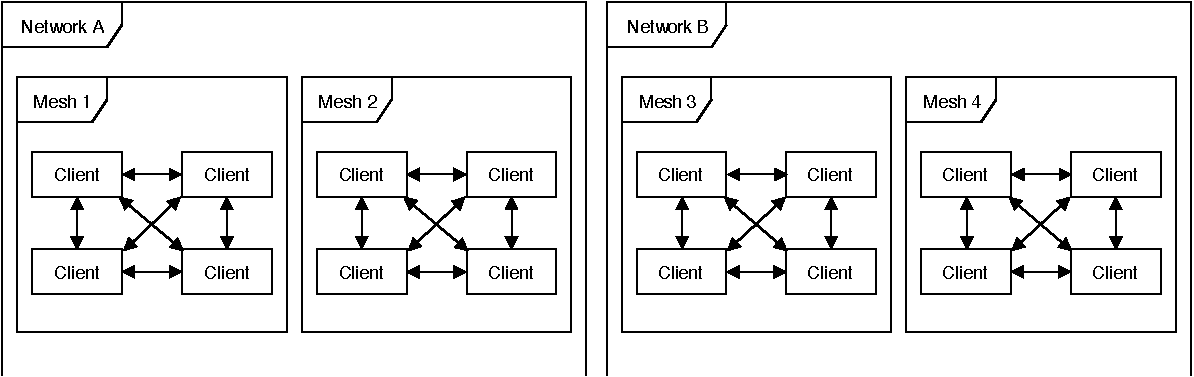
\includegraphics[width=0.8\textwidth]{figures/slidesync_peer_meshes}
	\caption[A Figure Short-Title]{Peer to Peer Meshes - Slidesync}
	\label{fig:mesh-slidesync}
\end{figure}


%Analyse workload
%
%Live Streaming
%- Event basiert
%- interessante Inhalte zum Teilen: Video stream
%- Viele Nutzer pro Event seite
%- aufsplittung von Peers anhand von lokalen Netzwerken wenn verfügbar

% voll vermaschtes netz
% mit bild
% Nutzung des anwendungswissens
% ip subnetz plus gleicher Kurs/stream


\section{Objekt Zuordnung - finden von Ressourcen}

Um das \pTp Netzwerk als \cdn Nutzbar zu machen ist es wichtig das ein Peer in der Lage ist herauszufinden wer welche resource bereitstellt. Dazu lassen sich verschiedene Ansätze verfolgen.

DHT\todo{distributed hash tables erklären}

Structured vs untructured

Da das Routing von Ressourcen bei den Betrachteten Anwendungsfällen in einem Zeitkritischen Moment erfolgen muss wurde sich für einen anderen Ansatz entschieden. Jeder Peer hält eine Hashtabelle mit den Ressourcen seiner Peers vor. Fügt ein Peer eine neue Ressource zu seinem Cache hinzu oder entfernt sie muss er alle verbundenen Peers über diese Änderung informieren. Dadurch muss im Falle einer Anfrage nicht erst die Ressource im Netzwerk gesucht werden. Dies ist möglich durch die Struktur des Netzwerkes. Da nicht alle Peers miteinander verbunden sind sondern voll vermaschte sub-meshes gebildet werden ist es möglich alle relevanten Peers über Änderungen zu informieren. Dadurch ist es möglich die Rechenleistung für das auffinden von Ressourcen in einen weniger Zeitkritischen Moment zu verlagern. Jedoch hat dies zur Folge das die Meshes so gebildet werden müssen das die Peers möglichst viele Ressourcen gemeinsam benötigen. Ist eine Ressource nicht im Mesh vorhanden kann sie vom Server geladen werden. 


%Structured vs unstructured networks
%
%Kollaborative File Sharing Protokolle wie z.B. Bitorrent verwenden häufig verteilte Hashtabellen zum auffinden von Ressourcen im Netzwerk. 
%Zhang proposed a DHT based P2P resource pool, SOMO
%[22], [23] to manage global resources and optimize multiple
%ALM (Application Layer Multicast) sessions,

%server hält liste vor --> kommunikation mit server nötig. \study
%
%peer fragt im Netzwerk an --> mehr kommunikation wenn in zeitkritischem moment \study
%
%peer halten liste von requests aktuell. Kommunikationsoverhead in zeitunkritischem moment \study
%	 peer weiß immer bei wer welche resource hat

% evtl diskussion verschiedener methoden 
%   server hält liste vor --> kommunikation mit server nötig
% peer fragt im Netzwerk an --> mehr kommunikation wenn in zeitkritischem moment
% peer halten liste von requests aktuell
%    kommunikationsoverhead in zeitunkritischem moment
%	 peer weiß immer bei wer welche resource hat
% am Anfang wird die zuordnung von einem peer an den neuen geschickt


\subsection{Subnetzerkennung}
\subsection{ Struktur von IP Adressen}
eher Konzept


\section{Wiederverwendbarkeit}
%Plug and play
%Konfigurierbarkeit
%einfaches einbinden in existierende anwendungen über npm
%javascript modul
%support von eigenen oder öffentlichen stun servern
%%Plug and play
\section{Open Source}
%was ist open source
%bereitstellung für die öffentlichkeit
%
